\capitulo{4}{Técnicas y herramientas} \label{cap:tecHerra}
En esta sección se explicarán las herramientas que se han puesto en práctica para la realización de este proyecto. 

\section{Python}
Este proyecto se ha desarrollado sobre \textit{Python}, un lenguaje de programación de alto nivel, multiplataforma, código abierto y dinámicamente tipado. Es uno de los lenguajes más usados en ámbitos como \textit{Data mining, Data science, Data analytics, Big Data, Inteligencia Artificial y Machine learning}

\section{Jupyter Notebook}
Los cuadernos de \textit{Jupyter} son considerados una aplicación online, diseñados para promover una computación interactiva. Pueden contener código, texto, material multimedia y ecuaciones. Por su gran versatilidad pueden ser utilizados en distintos ámbitos y sus usos más frecuentes son la exposición de resultados y datos, simulación numérica y modelado estadístico.

\section{Visual Studio Code}
\textit{Visual Studio Code} es un editor de código fuente, proporciona una gran cantidad de opciones para depurar código, permite trabajar con una amplia cantidad de lenguajes de programación como pueden ser \textit{C++, HTML, Java, JavaScript, PHP, R, Python o SQL} entre muchos otros. 
Además cuenta con la opción de poder tener una plataforma de control de versiones integrada en el editor.

\section{Git}
\textit{Git} es un \textit{software} de control de versiones de código abierto. Este tipo de sistemas son muy útiles a la hora de organizar proyectos ya que informan al usuario sobre los diferentes cambios realizados.

\section{Github}
\textit{Github} es una plataforma \textit{online} que permite alojar código de varios proyectos en un mismo repositorio usando el control de versiones \textit{Git}.

\section{\LaTeX}
\LaTeX es un sistema de composición de textos diseñado principalmente para la creación de documentos con una alta calidad tipográfica ~\cite{wiki:latex}. 

\section{Overleaf}
\textit{Overleaf} es un editor de \LaTeX de código abierto. Integra una amplia variedad de herramientas para poder redactar, editar y publicar documentos en línea. Es una herramienta muy sencilla de utilizar poniendo a disposición del usuario una compilación automática de manera que se puedan ir observando los cambios efectuados a medida que se realiza el documento. 

\section{Librerías de Python} \label{cap:librerias}
\subsection{NumPy}
\textit{NumPy} es una biblioteca de \textit{Python} que está especializada en el análisis de datos y en el cálculo numérico, tanto para grandes como para pequeños volúmenes de datos. 

\subsection{Pandas}
\textit{Pandas} ~\cite{mckinney2011pandas} es una biblioteca de \textit{Python} escrita como extensión de NumPy utilizada para el análisis y la manipulación de datos. Hay que destacar que es una librería muy cotizada para la manipulación de series temporales.

\subsection{Tslearn} \label{cap:tslearn}
\textit{Tslearn} ~\cite{tavenard2020tslearn} es un paquete de \textit{Python} con varias dependencias, utiliza las bibliotecas \textit{Numpy} y \textit{Scipy} para las manipulaciones de los datos de tipo matriz, las bibliotecas \textit{scikit-learn, Cython y joblib} para un cálculo eficiente y finalmente \textit{keras y tensorflow}. 

Este paquete permite la manipulación de conjuntos de datos de series temporales, tanto unidimensionales como multidimensionales, permitiendo el preprocesamiento de estos datos y la extracción de características.

En el ejemplo que se muestra en la figura \ref{fig:ts1} se puede observar como se crea un patrón de referencia denominado \textit{serie2} y a partir de unos valores aleatorios se obtiene una serie temporal de mayor mayor tamaño denominada \textit{serie1} que contiene al patrón de referencia.
El objetivo de este ejemplo es mostrar como el algoritmo puede extraer a la perfección el patrón de referencia dentro de la secuencia de mayor tamaño.

\begin{figure}[H]
    \centering
    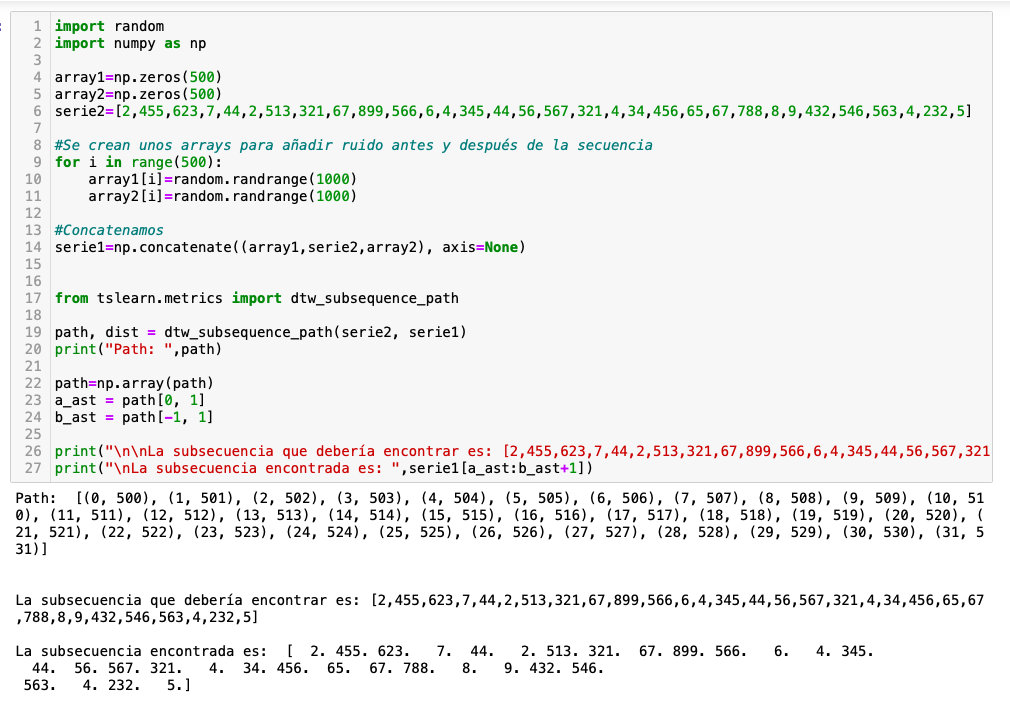
\includegraphics[width=\textwidth]{plantillaLatex-master/img/Example_Tslearn.png}
    \caption{ Ejemplo del uso de la librería \textit{tslearn}.}
    \label{fig:ts1}
\end{figure}


\subsection{dtaidistance}
\textit{Dtaidistance} ~\cite{wiki:dt1} es una biblioteca de \textit{Python} compatible con \textit{Numpy y Pandas} está destina al uso de datos de series temporales, como es el caso de la Deformación Dinámica de Tiempo (DTW, Dynamic Time Warping).En la figura \ref{fig:dta1} se puede observar un ejemplo que muestra como representar dos series temporales y su alineación \emph{DTW}.

\begin{figure}[H]
    \centering
    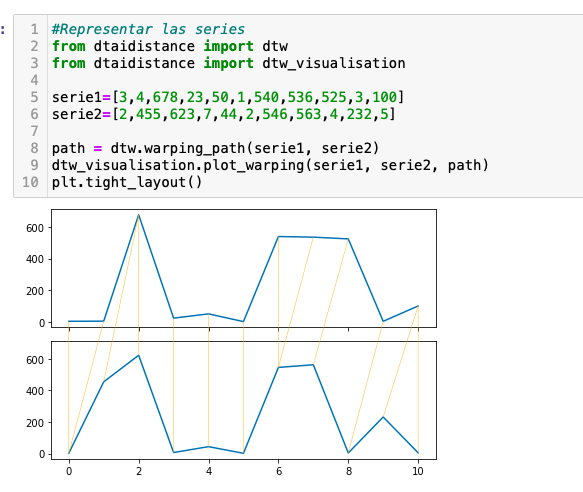
\includegraphics[width=\textwidth]{plantillaLatex-master/img/Example_dtaidistance.png}
    \caption{Ejemplo del uso de la librería \textit{dtaidistance}.}
    \label{fig:dta1}
\end{figure}


\subsection{pydtw}
\textit{pydtw} ~\cite{wiki:pydtw1} es una biblioteca de \textit{Python} utilizada para las alineaciones \emph{Dynamic Time Warping}. Esta librería se caracteriza por contener diferentes funciones para el análisis de series unidimensionales y multidimensionales, para el análisis de las primera se usa la función \textbf{dtw1d} y para las segundas la función \textbf{dtw2d}. En las figuras \ref{fig:dtw1d} y \ref{fig:dtw2d} se pueden observar un par de ejemplos de como utilizar estas funciones. 

\begin{figure}[H]
    \centering
    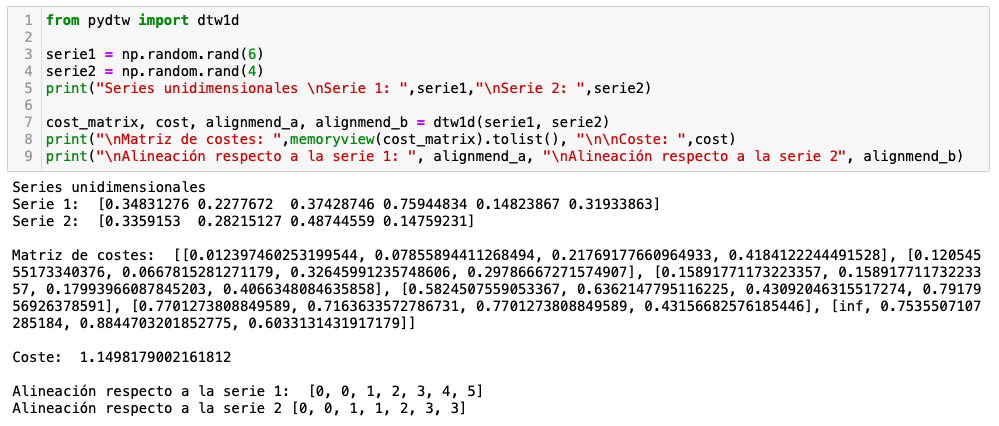
\includegraphics[width=\textwidth]{plantillaLatex-master/img/Example_pydtw_dtw1d.png}
    \caption{Ejemplo de uso de la función \textbf{dtw1d}.}
    \label{fig:dtw1d}
\end{figure}

\begin{figure}[H]
    \centering
    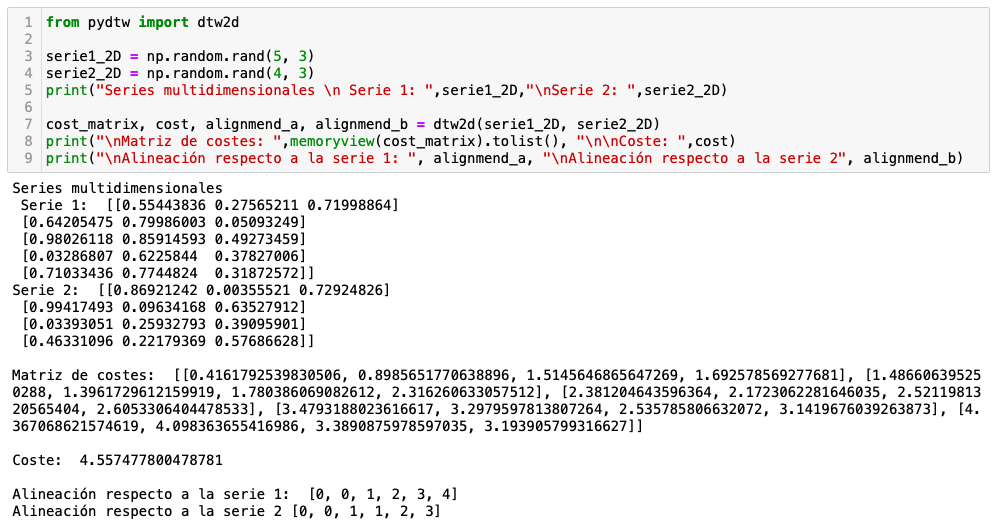
\includegraphics[width=\textwidth]{plantillaLatex-master/img/Example_pydtw_dtw2d.png}
    \caption{Ejemplo de uso de la función \textbf{dtw2d}.}
    \label{fig:dtw2d}
\end{figure}


\subsection{simpledtw}
\textit{simpledtw} es una biblioteca de \textit{Python} que cuenta con una implementación dinámica del algoritmo \emph{Dynamic Time Warping}. En la figura \ref{fig:simp} se muestra un ejemplo se puede observar como a partir de dos series, la función nos devuelve la mejor ruta de alineación entre ambas, el coste de esta alineación, dos listas que contienen los índices de cada una de las series con los que han sido emparejados respecto a la otra serie temporal, y finalmente, una matriz de costes.

\begin{figure}[H]
    \centering
    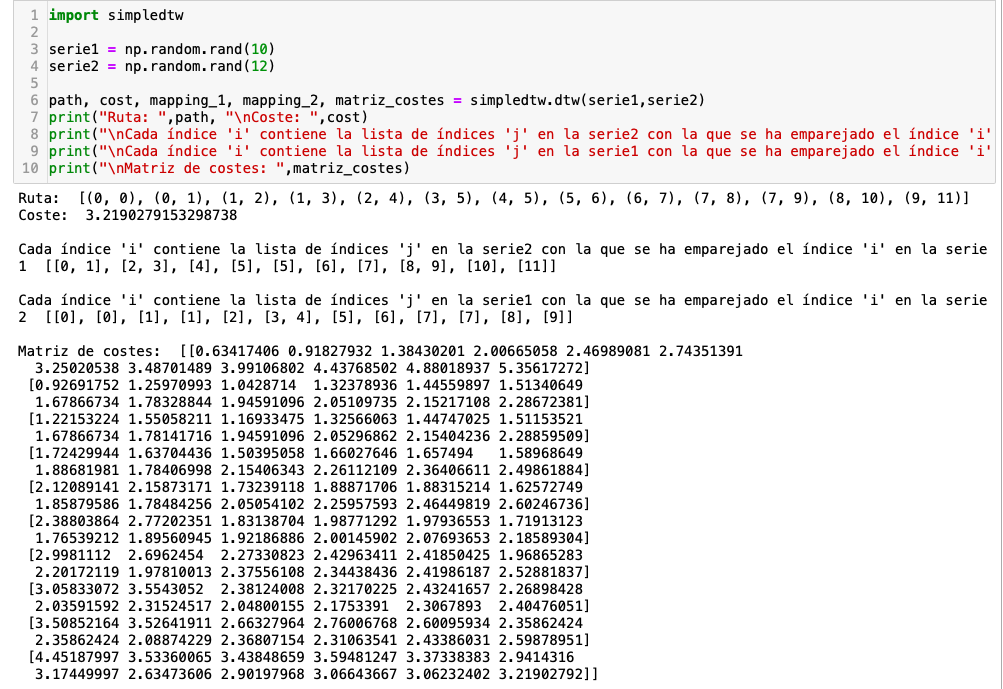
\includegraphics[width=\textwidth]{plantillaLatex-master/img/Example_simpledtw.png}
    \caption{Ejemplo del uso de la librería \textit{simpledtw}.}
    \label{fig:simp}
\end{figure}

\subsection{scipy}
\textit{scipy} es una biblioteca libre y de código abierto compuesta por una multitud de herramientas y algoritmos matemáticos. De esta biblioteca se extrae la función \textbf{scipy.signal.findpeaks} con la que pueden localizar picos dentro de una señal o secuencia. 

\subsection{Tkinter}
\textit{Tkinter} ~\cite{beniz2016using} es un paquete de \textit{Python} que proporciona la interfaz \textbf{TK}. Esta herramienta \textit{TK} nos permite desarrollar aplicaciones de escritorio multiplataforma, esto hace referencia a aplicaciones con una interfaz gráfica para distintos sistemas operativos, como Linux, Mac y Windows. 

\newpage
\section{Detectron}
\textit{Detectron} es una plataforma de detección de objetos creada por \textit{Facebook}. Su objetivo es dar suministro a la sociedad con código de gran calidad y buen rendimiento que se pueda emplear en el ámbito de la investigación de detección de objetos ~\cite{wiki:Detectron2018}.

Algunos de los algoritmos de detección de objetos que \textit{Detectron} incorpora son los siguientes:
\begin{enumerate}
    \item \textbf{Mask R-CNN}, es una ampliación de \textit{R-CNN más rápido}. Este modelo genera cuadros delimitadores y máscaras de segmentación para cada objeto localizado de la imagen ~\cite{dollar2017mask}.
    \item \textbf{RetinaNet}, este detector esta compuesto por una única capa, aspecto que lo hace más rápido pero algo menos preciso que otros detectores ~\cite{lin2017focal}.
    \item \textbf{R-CNN}: Este detector descompone una imagen y hace que estas descomposiciones entren, de forma secuencial, a una red convolucional que se encarga de la clasificación de los distintos objetos añadiéndoles una cierta probabilidad. El inconveniente es que este detector carece de rapidez de procesamiento. Para más información sobre las redes neuronales convolucionales, visitar el apartado \ref{cap:convolucional}. 
    \item \textbf{R-CNN rápido}, este detector crea dos procesos que pueden ser ejecutados de forma paralela. Por una parte se extraen las características de la imagen y por otra parte se descompone. Finalmente se realiza una proyección de las descomposiciones de la imagen sobre las características extraídas y se hace una clasificación por cada una de ellas.
    \item \textbf{R-CNN más rápido}, este detector funciona con la misma lógica que el detector anterior con la diferencia de que las descomposiciones de la imagen se realizan una vez extraídas las características de la imagen ~\cite{ren2015faster}. 
    \item \textbf{R-FCN}, este detector esta basado en regiones y es totalmente convolucional con un cálculo compartido en la plenitud de la imagen. 
\end{enumerate}

\section{Detectron2} \label{cap:Detectron2}
Esta biblioteca es la evolución de \textit{Detectron} y \textit{ maskrcnn-benchmark} y proporciona algoritmos de detección de objetos de última generación. Una de sus características principales frente al modelo anterior, es que consigue entrenar los datos mucho más rápido ~\cite{wu2019detectron2}. Para mostrar al usuario lo versátil que pueden ser la herramienta \textit{Detectron2} se han creado una serie de imágenes en las que se pueden ver como identifica a diferentes animales, vehículos e individuos. 

Como primer comienzo se mostrará una sencilla clasificación de animales usando diferentes algoritmos de detección de objetos. En la figura \ref{f:animales1} se puede observar como detecta a la perfección los distintos tipos de animales que aparecen en cada fotografía. 

\begin{figure}[H]
 \centering
  \subfloat[\textit{faster\_rcnn\_R50DC51x}]{
   \label{f:gatos}
    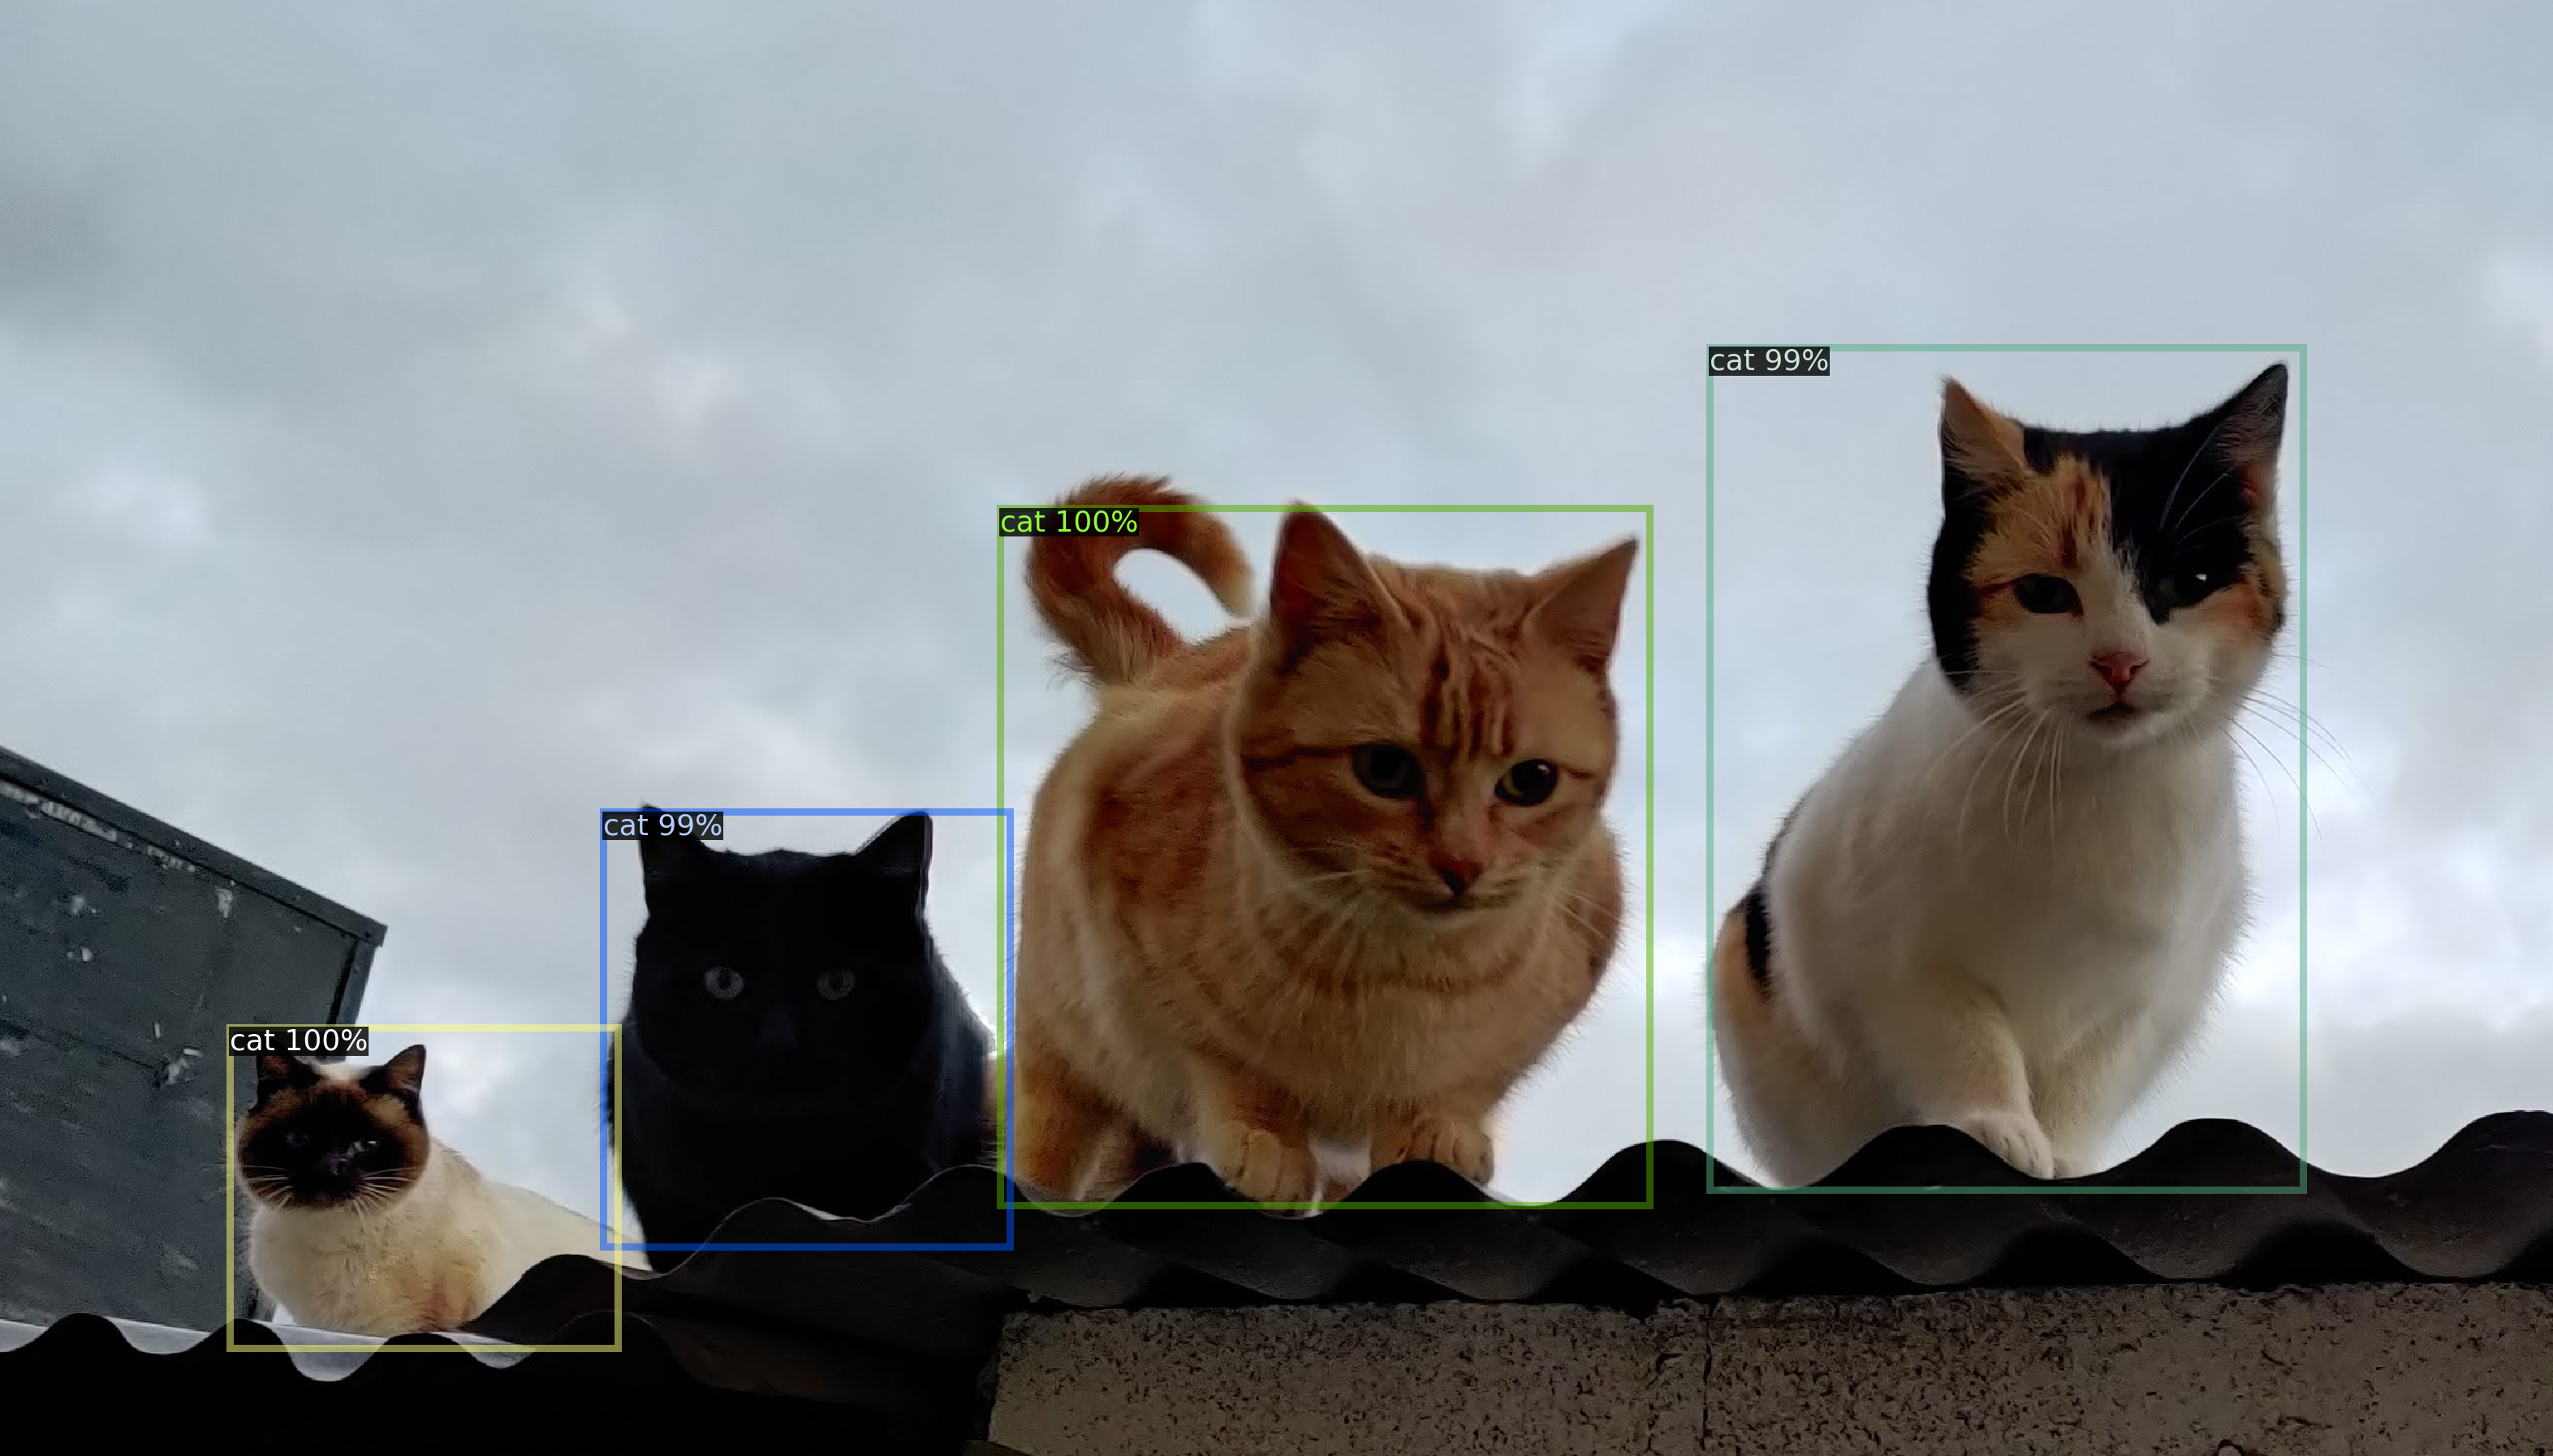
\includegraphics[width=0.35\textwidth]{faster_rcnn_R_50_DC5_1x.png}}
  \subfloat[\textit{faster\_rcnn\_X10FPN3x}]{
   \label{f:perros}
    \includegraphics[width=0.32\textwidth]{faster_rcnn_X_101_32x8d_FPN_3x.png}}
  \subfloat[\textit{faster\_rcnn\_R50FPN1x}]{
   \label{f:loros}
    \includegraphics[width=0.30\textwidth]{faster_rcnn_R_50_FPN_1x.png}}
 \caption{Detección de animales usando diferentes algoritmos.}
 \label{f:animales1}
\end{figure}

Subiendo un poco más el nivel, en la figura \ref{f:animales2} se pueden observar un par de imágenes que contienen un mayor número de objetos, individuos y animales. En la primera imagen el algoritmo detecta al elefante, a los individuos que salen en ella, e incluso el objeto que porta el animal. Por consiguiente, en la segunda imagen, se puede apreciar como detecta a la perfección a las personas que se encuentran sentadas. Claramente se ven muy borrosas por el desenfoque de la imagen pero aun así, el algoritmo las identifica con un 94\% y 96\% de precisión. 

\begin{figure}[H]
 \centering
  \subfloat[\textit{mask\_rcnn\_R101DC53x}]{
   \label{f:elefante}
    \includegraphics[width=0.29\textwidth]{mask_rcnn_R_101_DC5_3x.png}}
  \subfloat[\textit{faster\_rcnn\_R50FPN\_noaug\_1x}]{
   \label{f:perros}
    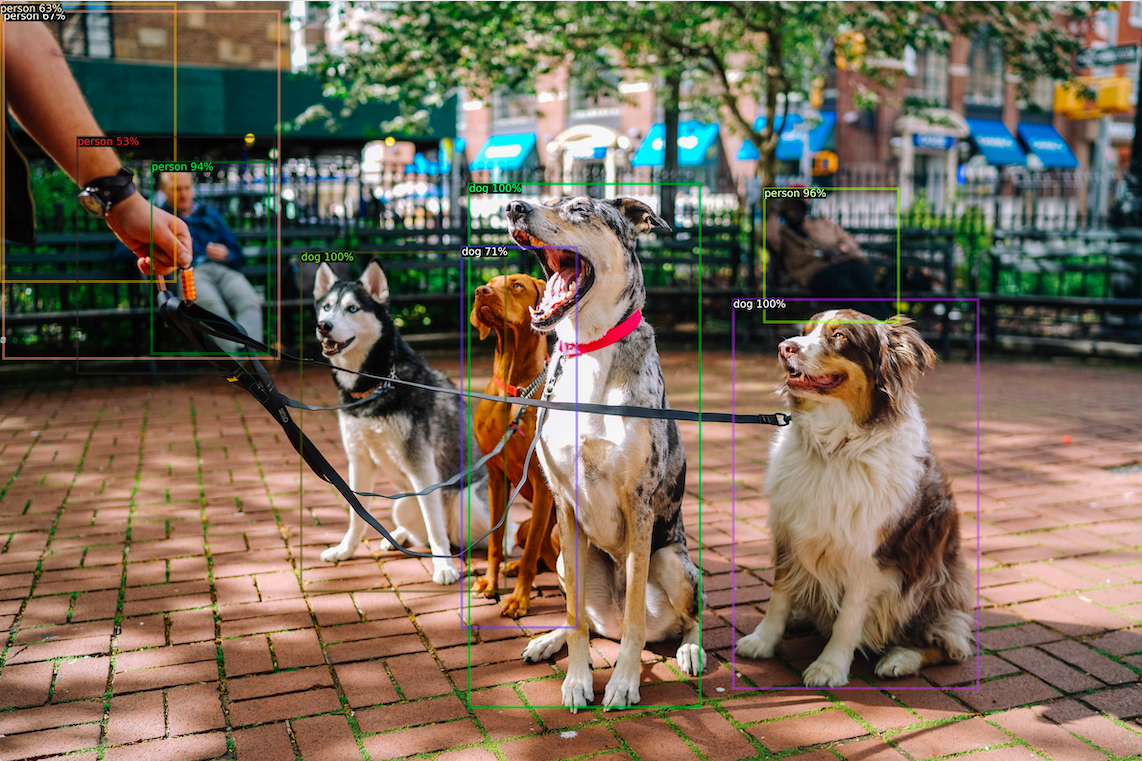
\includegraphics[width=0.65\textwidth]{plantillaLatex-master/img/faster_rcnn_R_50_FPN_noaug_1x.png}}
 \caption{Detección de diferentes objetos usando varios algoritmos.}
 \label{f:animales2}
\end{figure}

Finalmente en la figura \ref{f:f_esq}, se mostrarán unas imágenes más relevantes al objeto de estudio de este proyecto. En ella se puede observar como mediante la implementación de distintos algoritmos de detección de objetos se ha podido extraer el esqueleto de los distintos individuos de las imágenes. 

\textit{Detectron2} es capaz de localizar los diferentes objetos de la imagen y los algoritmos de detección de poses son capaces de extraer varios esqueletos de una misma imagen. Por ello en la figura \ref{f:f_esq2} se pueden observar varios individuos y sus correspondientes esqueletos. Cabe destacar, que si los individuos están demasiado alejados, o si no se les puede detectar completamente, habrá imprecisión a la hora de extraer los esqueletos. 

\begin{figure}[H]
\centering
  \subfloat[\textit{keypoint\_rcnn\_R\_50\_FPN\_3x}]{
   \label{f:f}
    \includegraphics[width=0.54\textwidth]{keypoint_rcnn_R_50_FPN_3x.png}}
  \subfloat[\textit{keypoint\_rcnn\_X\_101\_FPN\_3x}]{
   \label{f:f}
    \includegraphics[width=0.48\textwidth]{keypoint_rcnn_X_101_32x8d_FPN_3x.png}}
 \caption{Detección de esqueletos.}
 \label{f:f_esq2}
\end{figure}


\begin{figure}[H]
 \centering
  \subfloat[\textit{faster\_rcnn\_faster\_rcnn\_R\_101\_FPN\_3x}]{
   \label{f:faster1}
    \includegraphics[width=9cm]{plantillaLatex-master/img/faster_rcnn_R_101_FPN_3x.png}}\vspace{1mm}
  \subfloat[\textit{mask\_rcnn\_R\_50\_FPN\_1x}]{
   \label{f:faster2}
    \includegraphics[width=9cm]{mask_rcnn_R_50_FPN_1x.png}}\vspace{1mm}
  \subfloat[\textit{keypoint\_rcnn\_R\_50\_FPN\_1x}]{
   \label{f:faster3}
    \includegraphics[width=9cm]{keypoint_rcnn_R_50_FPN_1x.png}}
 \caption{Detección de esqueletos usando diferentes algoritmos.}
 \label{f:f_esq}
\end{figure}


\newpage
\section{Máquinas Virtuales Dockers}
\emph{Docker} es un proyecto software que proporciona una tecnología de virtualización basada en contenedores y por lo tanto, una virtualización a nivel de sistema operativo. A diferencia de las \textit{Máquinas Virtuales}, los contenedores no albergan un sistema operativo completo, si no que comparten los recursos del sistema sobre el que se ejecutan, reutilizando reutilizan el hardware y el kernel de la máquina sobre la que se hospedan. En la figura \ref{fig:M-V} se puede interpretar la diferencia entre la estructura de una \textit{Máquinas Virtuales} y un \textit{contenedor Docker} ~\cite{docker}.

\begin{figure}[H]
    \centering
    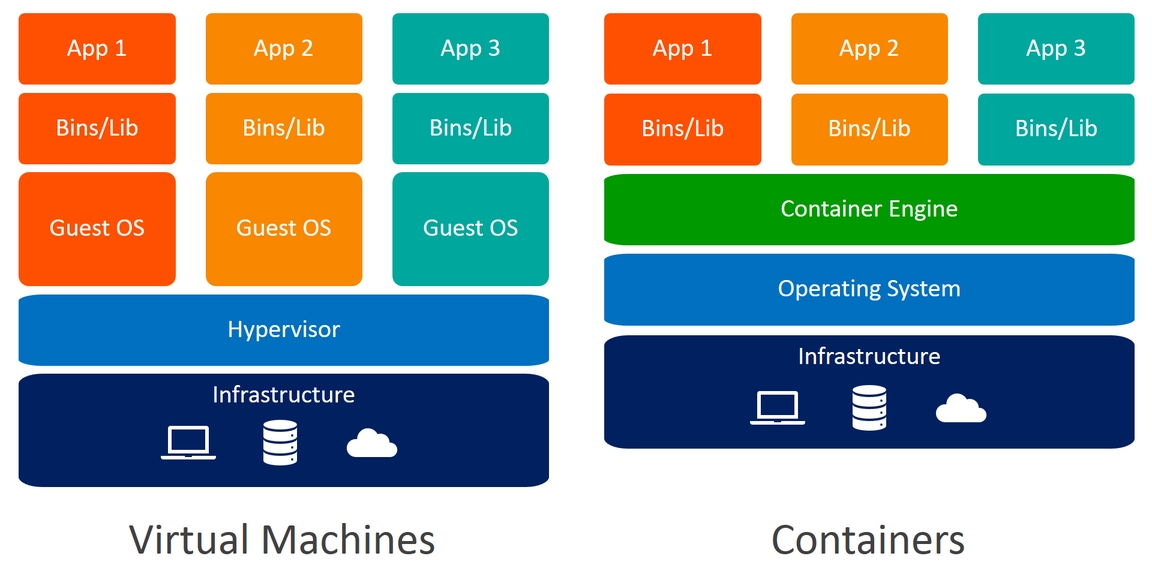
\includegraphics[width=\textwidth]{plantillaLatex-master/img/DockerVsMv2.jpg}
    \caption{Contenedor \textit{Docker} vs Máquinas Virtuales.}
    \label{fig:M-V}
\end{figure}


Esta tecnología tiene como ventaja la posibilidad de poder desarrollar una aplicación, probarla y ejecutarla desde distintos dispositivos sin tener que perder demasiado tiempo en adaptar el entorno a la aplicación requerida.

Los \textit{contenedores Docker} usan la arquitectura cliente-servidor. El \textit{cliente Docker} se comunica con el demonio de \textit{Docker} a través una \textit{API REST}, una interfaz de red o mediante un \textit{sockets UNIX}. Esta comunicación se realiza para poner en marcha las tareas encomendadas como pueden ser, ejecutar un contenedor o compilar una serie de \textit{imágenes Docker}. Otro cliente con el que cuenta \textit{Docker} es \textit{Docker Compose} que proporciona la posibilidad de poder trabajar con aplicaciones basadas en un conjunto de contenedores.En la figura \ref{fig:C-S} se puede observar una representación de esta arquitectura.

\begin{figure}[H]
    \centering
    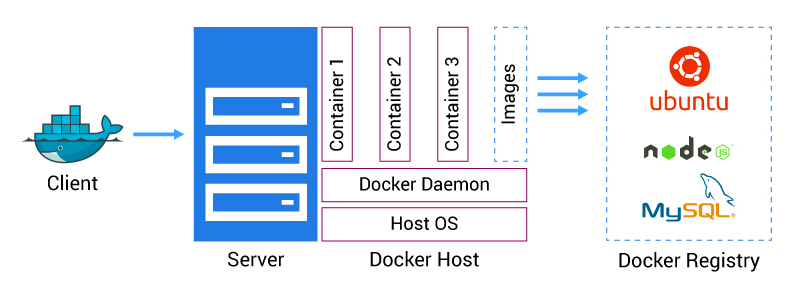
\includegraphics[width=\textwidth]{plantillaLatex-master/img/DockerClientServer.png}
    \caption{Estructura Cliente-Servidor \textit{Docker}.}
    \label{fig:C-S}
\end{figure}

\begin{figure}[H]
    \centering
    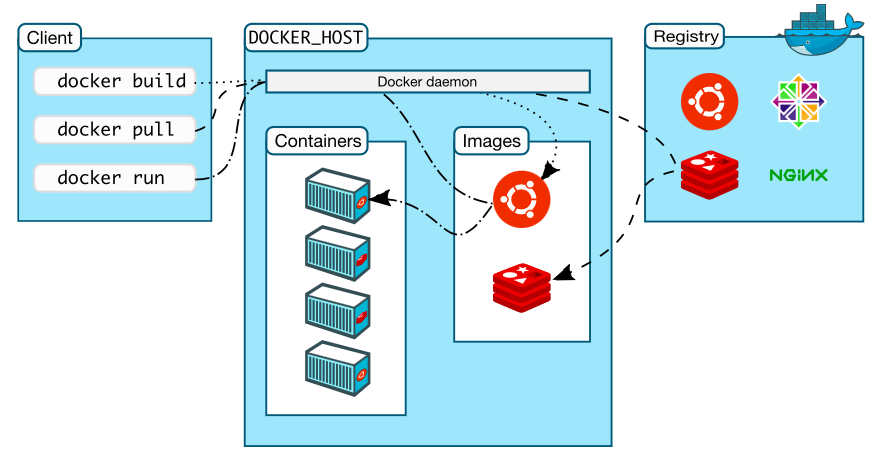
\includegraphics[width=\textwidth]{plantillaLatex-master/img/DockerArchitecture.png}
    \caption{Arquitectura \textit{Docker}.}
    \label{fig:ArquitecturaD}
\end{figure}

Para entender la arquitectura de \textit{Docker} se dará una breve introducción a los componentes principales, que se muestra en la figura \ref{fig:ArquitecturaD}:
\begin{enumerate}
    \item \textbf{Demonio Docker}, se encarga de atender las peticiones de la \textit{API} y manejar los objetos \textit{Docker} como pueden ser las imágenes o los contenedores. Esto demonios también pueden comunicarse entre sí.
    \item \textbf{Cliente Docker}, es la manera que tiene el usuario de interactuar con el Docker. Por ejemplo, en la imagen \ref{fig:ArquitecturaD} se puede observar como el cliente usa los siguientes comandos:
    \begin{enumerate}
        \item \textit{docker build}, es el encargado de permitir al usuario la creación de imágenes Docker.
        \item \textit{docker pull}, una vez creada la imagen, este comando permite que sea descargada, por defecto descargará la última imagen creada aunque se puede especificar la imagen que se desea descargar
        \item \textit{docker run}, finalmente con este comando se crea un contenedor a partir de la imagen indicada y lo pone en funcionamiento.

\begin{figure}[H]
    \centering
    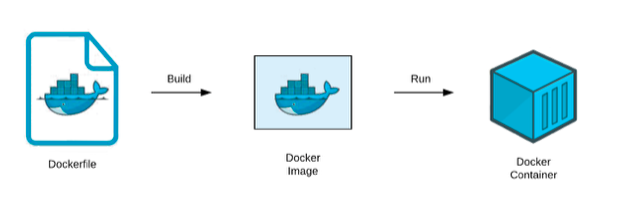
\includegraphics[width=0.8\textwidth]{plantillaLatex-master/img/DockerRunBuild.png}
    \caption{Ejecución contenedor \textit{Docker}.}
\end{figure}

    \end{enumerate}
    \item \textbf{Motor Docker}, permite que sea posible ejecutar los distintos contenedores y las imágenes \textit{Docker}. 
    \item \textbf{Docker Hub}, es un repositorio en el que los usuarios pueden participar compartiendo sus propias imágenes y contenedores \textit{Docker} o adquiriendo los que proporcione la comunidad \textit{Docker}. 
    \item \textbf{Imágenes Docker}, son identidades de software autosuficientes con instrucciones para la creación de contenedores. Para su creación, se empezará creando un \textit{Dockerfile} compuesto por una serie de instrucciones. Cada una de estas instrucciones creará una capa en la imagen. Estas capas hacen que al modificar el \textit{Dockerfile} y reconstruir las imágenes, sólo se reconstruyan las capas que han sido modificadas, haciendo que las imágenes sean tan ligeras pequeñas y rápidas comparadas con otras tecnologías de virtualización.
    \item \textbf{Contenedor Docker}, un contenedor es una instancia ejecutable de una imagen. Están definidos por estas imágenes y por defecto suelen permanecer aislados de su máquina \textit{host} o de otros contenedores.Se pueden realizar varias acciones sobre ellos utilizando la \textit{API} o la \texttt{CLI}\footnote{CLI es una interfaz de línea de comandos (en inglés,command-line interface) que permite a los usuarios escribir comandos a algún programa o al sistema operativo por medio de una línea de texto simple } como pueden ser:
    \begin{enumerate}
        \item Iniciar un contenedor, \emph{docker container start}.
        \item Detener un contenedor, \emph{docker container stop}. Los argumentos que se deben de pasar para que el contenedor se detenga, sería el nombre o el ID del contenedor. 
        \item Borrar un contenedor, \emph{docker container rm}. 
        \item Comprobar relaciones entre contenedores, \emph{docker container inspect}. Con este comando se puede consultar información de bajo nivel sobre un contenedor
        \item Ejecutar un comando en un contenedor en ejecución, \emph{docker container exec}. Este último comando ha sido muy útil para poder comprobar el correcto funcionamiento del programa.
    \end{enumerate}
\end{enumerate}

